\section{IO Ecosystem Specifics}
\label{sec:io}

\paragraph{Lightwallet.} HD wallets in Cardano are mostly BIP44-compatible
wallets, with the exception that the used elliptic curve is Ed25519,
instead of Secp256k1, like Bitcoin's BIP32 (and thus, BIP44). This
difference is marked by using index 1852 for hardened child derivation at
layer 1 (purpose level), as specified in CIP1852%
\footnote{\url{https://cips.cardano.org/cips/cip1852/}. Last access, December
  15th, 2021.}. Mnemonics in Cardano are composed by 24 words, and hence
encode 256-bit random bitstrings.

\paragraph{Atala.} HD wallets in Atala follow the same overall rules as in
BIP32. Specifically, the same distinction between hardened and non-hardened
child derivation rules are applied, as well as Secp256k1 as the elliptic curve,
wich ECDSA as digital signature scheme. However, Atala defines a different
tree structure, with the following layers, depicted also in \figref{fig:atalatree}:

\begin{description}
\item[Layer 0: Root.] Encoded as/derived from a 12-word mnemonic.
\item[Layer 1: DID Number.] Obtained by hardened child derivation from the root.
  Each node in this level corresponds to a different DID.
\item[Layer 2: Key Type.]  Obtained by hardened child derivation from a layer 1
  node. Currently, the Atala specification defines four types of keys: master
  keys, issuing keys, communication keys, and authentication keys.
\item[Layer 3: Index.] Obtained by hardened child derivation from a layer 2 node.
  Each layer 2 node may have up to $2^{31}$ child nodes, which are the leaves of
  the tree.
\end{description}

See the key derivation document for details%
\footnote{\url{https://github.com/input-output-hk/atala-prism/blob/master/prism-backend/docs/protocol/key-derivation.md}. Last access December 15th, 2021. \textbf{WARNING!
    Internal link!}}. Mnemonics in Atala are composed by 12 words, and hence
encode 256-bit random bitstrings.

\begin{figure}[ht]
  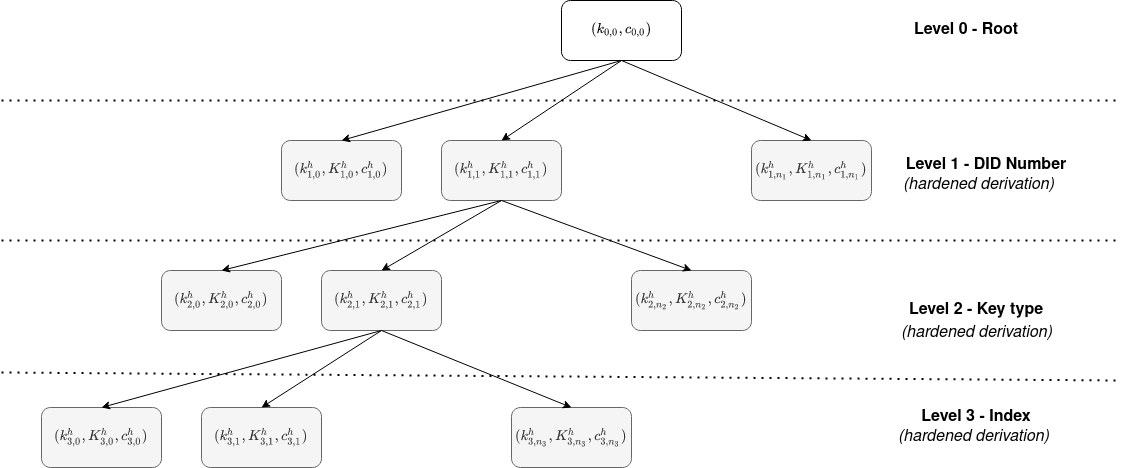
\includegraphics[width=\textwidth]{figures/atala_tree.png}
  \caption{Atala tree derivation structure.}
  \label{fig:atalatree}
\end{figure}

\paragraph{Related effots.} There seems to be an effort to analyse the security
of wallets that manage addresses combining payment and staking keys \cite{kkl20}.
These wallets are referred to as PoS wallets. The paper identifies a series of
malleability attacks, depending on how the addresses are derived from the
associated staking and payment keys. A core wallet functionality is proposed,
and a base protocol realizing that functionality is given. While the proposal
seems to be somehow compatible with BIP44 wallets, the proposal seems to be
somehow orthogonal to the way keys are derived -- instead, they focus on how
to generate addresses, and check that produced/received addresses are correct.

\subsection{Aspects to consider before unification}
\label{ssec:unification}

Next, we emphasize some concrete topics that would need to be considered
from an implementation/software-design point of view, prior to making
Atala and Cardano keys to be derived from a single mnemonic.

\paragraph{Domain separation when different cryptosystems is
  necessary.} %
As mentioned, Cardano uses EdDSA (which is based on Ed25519 curve),
while Atala uses ECDSA with Secp256k1. It is \emph{not} a good idea%
\footnote{I have not been able to find a paper that describes
  some concrete related attack or gives some impossibility result for
  proving security under this circumstance but, at the least, it seems to
  be folklore knowledge. See Lindell's answer at
  \url{https://crypto.stackexchange.com/a/54666/52362} for instance.
  \cite{dlp12+,thorm21} seem good references to study this topic further, if
  needed.} to use the same key in different cryptosystems, nor for different
curves, even though ``structurally'' it may be possible (e.g., in EdDSA and
ECDSA, private keys are 32-byte random numbers). However, this is easily
avoidable by ensuring domain separation in the key derivation functions that
are applied on the common seed. This is an important concern on its own; yet,
it should be addressed natively through the considerations in the next
paragraph.

\paragraph{Ensure a correct hierarchical key derivation strategy.} %
We need to take into account what specific usage we expect from the wallets
and, from there, define hierarchical derivation rules that ensure security
without disabling current utility. Related to the previous paragraph, we should
make sure that keys that are aimed to be used in different
cryptosystems, are derived in separate tree branches that ensure domain
separation. Or, since the Atala derivation path is shorter, than no Atala
derivation path can be a prefix of a Cardano derivation path. For instance,
according to the current specification, the derivation path
\texttt{m/1852'/1815'/0'} corresponds to account \texttt{0'} for Ada coins in
CIP1852-compliant Cardano wallets. In Atala, \texttt{1852'} could be a valid
DID number and, while \texttt{1815'} is currently not a valid key type, if,
in the future it becomes so, then \texttt{m/1852'/1815'/0'} would be a valid
derivation path in both Atala and Cardano -- which could open an attack vector.
An easy fix would be to concatenate the master seed with some value \texttt{C}
in Cardano, and some distinct value \texttt{A} in Atala. The derivation paths would
become \texttt{Cm'/1852'/1815'/...} in Cardano, and \texttt{Am'/...} in Atala
-- hence, domain separation would be ensured. Probably, many other alternatives
exist, more suitable from an engineering perspective (e.g., assigning Atala its
own \texttt{purpose} level in BIP44 wallets). But, whatever option is followed,
domain separation should be ensured.

\paragraph{On the mnemonic length.} %
Atala uses 12-word mnemonics to encode the master seed from which all keys are
derived, while Cardano uses 24 words. According to BIP39, 12 words encode 128-bits
seeds, and 24 words encode 256-bit seeds. These entropy bits are then subject to
the extract-and-expand approach of the HKDF used in BIP32 to produce pseudoranom
bits that are computationally indistinguishable from true random numbers%
\footnote{Note: only 256 of these bits are used to produce the final keys.}.
The keys used by both Atala (for ECDSA), and Cardano (for EdDSA), are thus
securely derived pseudorandom keys of 256 bits. For keys of 256 bits, both ECDSA
and EdDSA are expected to provide 128 bits of security against unforgeability
attacks. Given this, and assuming (like \cite{def+21} does) that some keys
will be compromised, there are two ways to attack a wallet: by breaking
security of the HKDF used to derive the keys; or by breaking security of
the wallet construction itself. Given this, on the one hand, in \cite{def+21}%
\footnote{Important! Note that \cite{def+21} is defined for ECDSA-based BIP32
  wallets with a structure slightly different from BIP44 wallets. Hence, its
  results may not translate to our setting -- and of course, neither to
  EdDSA-based BIP44 wallets.}, security of BIP32 wallets against unforgeability
is estimated to have a security loss of 37 bits over the underlying digital
signature scheme (under somewhat arbitrary estimations for
a typical setting, like leaking about $1\%$ of roughly $2^{20}$ produced
keys). For 256-bit ECDSA keys, this translates to 91 bits of security.
On the other hand, even for 128-bit seeds (thus, with entropy at most
128), breaking the security of the HMAC-based HKDF construction (that would
seem to affect the unlinkability property of BIP32 wallets, rather than their
unforgeability) would be harder than breaking the unforgeability property of
the BIP32 wallet, as per the results in \cite{kraw10}\footnote{According to the
  analysis in \cite{kraw10}, the outputs of HMAC-based HKDFs are roughly
  $q2^{-m}$-close to uniform, where $q$ in our setting would be $2^{20}$ as per
  \cite{def+21}, and $m$ is the min-entropy of the randomness source (our
  mnemonic). Hence, for seeds (mnemonics) of 128 bits of entropy, we can still
  expect the outputs to be $\sim 2^{-100}$-close to uniform.}. Given this, and
lacking a more detailed analysis, seeds of 12 words would appear to be enough
for security, strictly speaking. However, taking into account that we are
aiming to combine two wallets into one, it does not seem logical to reduce the
overall security of the wallet that uses 24-word mnemonics, as the unified
wallet will use the same mnemonic to produce even more keys than what it
was producing before. Therefore, it seems advisable to increase the mnemonic
length of Atala to 24 words, rather than reducing the length of Cardano to
12 words.

%%% Local Variables:
%%% mode: latex
%%% TeX-master: "single-mnemonic"
%%% End:
